\chapter{Technology architecture}
\label{sec:technology-architecture}

    This chapter covers the technology architecture (term from the ArchiMate language). It is used for modelling the underlying infrastructure and deployment of applications as software, servers, clusters, load balancers, etc. The next section presents a generic pattern which we substantiate in this architecture. 
    
	\section{Prototypical technology structure}
	
	This section presents a generic technology architecture organisation, depicted in Figure \ref{fig:technology-view}, in order to ease interpretation of the diagrams that follow.
	
	\begin{figure}[!h]
		\centering
		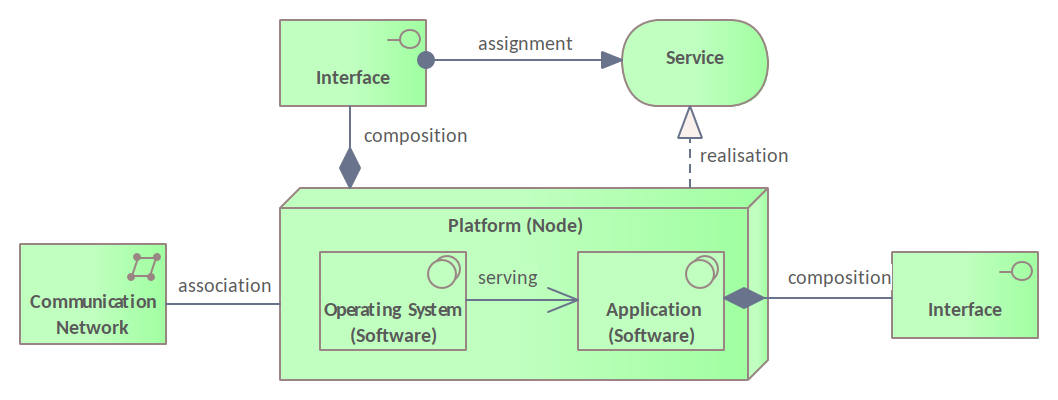
\includegraphics[width=.75\textwidth]{images/views/Technology View.png}
		\caption{The prototypical technology view}
		\label{fig:technology-view}
	\end{figure}

	The central concept in the technology view is the node. It represents a computational or physical resource that hosts, manipulates or interacts with other computational or physical resources. Within a node, various software components are deployed, most foundational of which is the operation system. The node aggregates various software. 
	
	Depending on the chosen level of granularity, nodes may realise technology services which represent explicitly defined and exposed behaviour. Also, nodes and software may expose interfaces which represent points of access where a technology service offered by a node can be accessed. Interfaces constitute parts of the node: an interface may be assigned to a service.
	
	Lastly, node are connected to the communication network which represents a set of structures that connects nodes for transmission, routing and reception of data. There may be one or more networks depending on the organisation security policies and on the internal infrastructure setup. These ArchiMate elements suffice to describe the current and new technology architectures. 	
	
	\section{Current technology architecture}
	\label{sec:technology-current}
	
	The current SU infrastructure necessary to support the application life-cycle is depicted in Figure \ref{fig:technology-current}. It comprises four nodes for a private network and a controlled connection to the internet. 
	
	\begin{figure}[!h]
		\centering
		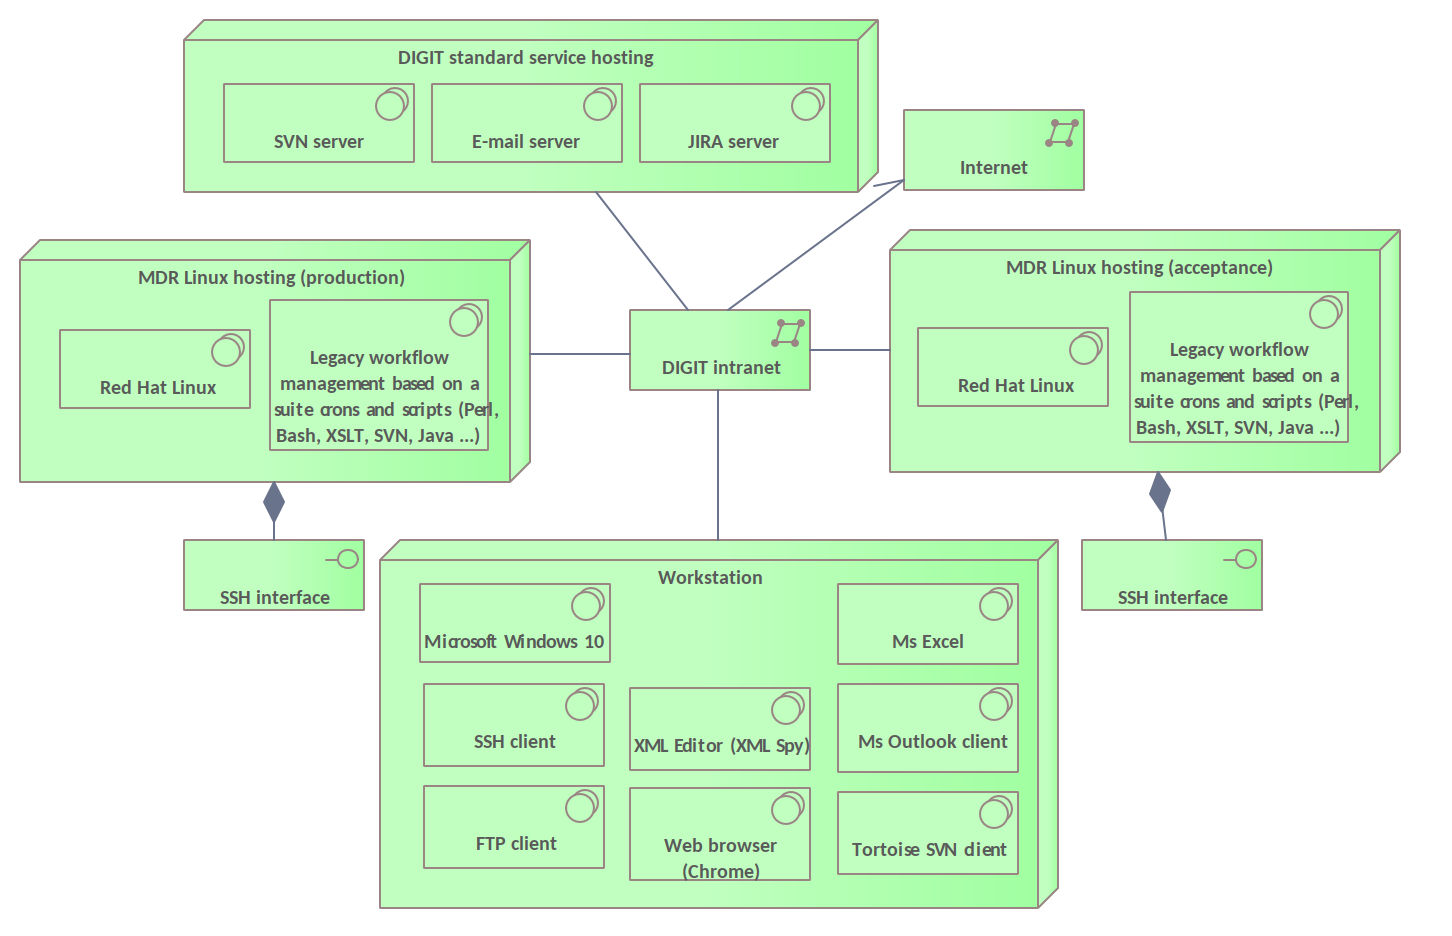
\includegraphics[width=1.01\textwidth]{images/technology/Current Platform.png}
		\caption{The technology structure that supports the current asset lifecycle}
		\label{fig:technology-current}
	\end{figure}
	
	At the bottom of the diagram is the workstation node which represents the standard machine provided to the members of the SU team by the DIGIT infrastructure unit. The workstation runs Windows 10 \citep{windows10} operating system and the following set of tools (at least) are installed on it: MS Excel, Outlook, Chrome (os another modern browser), an SVN client (Tortoise SVN is the default choice by the SU team), a specialised XML editor (XML Spy is the default), an FTP client of choice and an SSH client (Putty is the default). This set of software is used to perform all the necessary duties and enact the described business processes. 
	
	At the top of the diagram is depicted the standard service hosting offered by DIGIT. The provided services there are the e-mail service, a dedicated the SVN repository as a service and a set of Jira projects.
	
	In addition, two identically-housed Linux servers are provided: one acting as the acceptance environment and the second as the production environment. They are registered at DIGIT as ``MDR Linux hosting'' nodes and they host the legacy workflow management system. This legacy system is based on multiple technologies which were added gradually and organically in the course of its development. It includes components written as Perl scripts, Bash scripts, many XSLT transformation style-sheets, commends relying on existence of an SVN client and Java libraries and scripts.
		
	One of the MDR Linux hosting nodes serves for testing purposes and the other one an operational environment for production. The nodes run RedHat Linux 7.7 operating system and each expose an SSH interface. These interfaces are used by the technical team. The technical team member connect using SSH from their workstations and operate the legacy workflow management system remotely.
	
	The communication network is secured as an intranet-authenticated connection provided by DIGIT. From the intranet, a controlled access to the Internet is available through an authentication proxy. 
	
	This completes the description of the current infrastructure architecture and sets the baseline for the new architecture described in the next section.
	
	\section{New technology architecture}
	\label{sec:technology-new}
	
	The new infrastructure architecture is depicted in Figure \ref{fig:technology-new}. What are the same as in the current one are the structure of the workstation node, the intranet and the Internet connections, as well as standard hosted services to which are added VocBench3 and the Adobe FrameMaker server which are necessary for realising the asset description documentation (ADD) service, in addition to a few other important services within SU, among which is the generation of the Interinstitutional Style Guide. 
	
	\begin{figure}[!h]
		\centering
		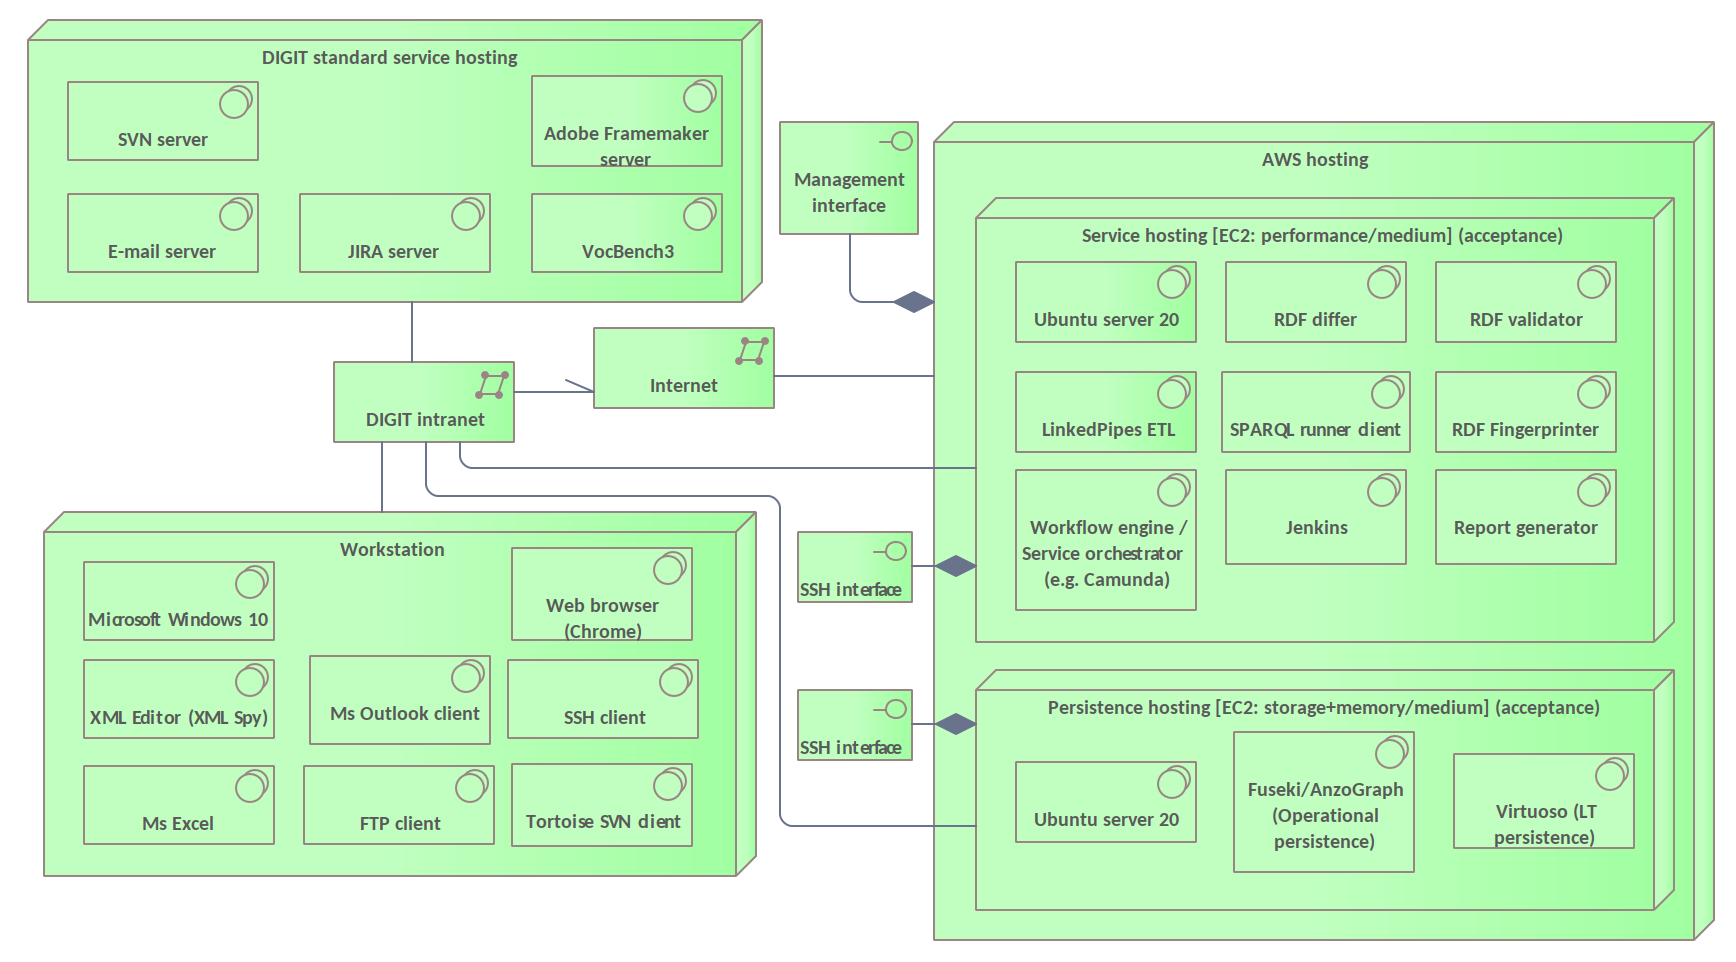
\includegraphics[width=1.01\textwidth]{images/technology/New Platform.png}
		\caption{The technology structure that supports the new asset lifecycle}
		\label{fig:technology-new}
	\end{figure}

	What differs significantly between the two is the disappearance of the hosted nodes (left and right side of Figure \ref{fig:technology-current}) and their replacement with dedicated Amazon Web Service (AWS) hosting, depicted as a large node on the right side of Figure \ref{fig:technology-new}. This node exposes a management interface which provides the possibility of configuring and launching multiple virtual servers (called EC2 instances) of various sizes and performance capabilities. This puts an administration overhead onto the SU team, but also frees it from a large number of constraints and experiences in the past years, this way smoothing the path for this and future digital transformations.
	
	In the new architecture, to support the application architecture described in Section \ref{sec:application-architecture}, two instances are necessary: one optimised for performance and another optimised for persistence. The first one hosts the operational application components, while the second one hosts the triple stores and potentially other types of databases. This initial separation into two could be further optimised by moving some services to dedicated EC2 instances if deemed necessary. Also, these two instances are considered an acceptance environment where the new application is assembled and tested. Once it is ready to move into production, an identical copy of EC2 instances is created and those are further used for production operations. 
	
	The EC2 instance at the top, marked for performance, runs a Linux OS, preferably Ubuntu 20 or RedHat 8, and has installed the following software: RDF differ (custom-built component), RDF validator (custom-built component), RDF fingerprinter (custom-built component), LinkedPipes ETL, Jenkins automation system and optionally Camunda BPM. 
	
	The EC2 instance at the bottom, marked for persistence, needs to run Ubuntu or RedHat as well, and hosts triple stores: Fuseki (for the custom built components) and for LinkedPipes ETL, which are optimised for operational performance, and an instance of Virtuoso triple store which is meant for long-term preservation of RDF data. 
	Optionally, in the acceptance phase, the triple stores could be hosted on a single EC2 instance to avoid management overheads. 
	
	Each of the EC2 instances expose an SSH interface which can be accessed by the technical team to configure, manipulate and operate the servers, just like in the currently-hosted MDR Linux server. 
	